\documentclass[12pt,fleqn,handout]{beamer}


\xdefinecolor{lavendar}{rgb}{0.8,0.6,1}
\xdefinecolor{olive}{cmyk}{0.64,0,0.95,0.4}
%\xdefinecolor{olive}{cmyk}{1,0,0,0}
\xdefinecolor{mag}{cmyk}{0.1,1,0,0.2}
\xdefinecolor{lblue}{rgb}{0,0,1.5}
\xdefinecolor{lred}{rgb}{1,0,0}
\xdefinecolor{mine}{cmyk}{1,0,0.2,0}
\xdefinecolor{bluel}{cmyk}{0.1,0,0.9,0.4}

\usepackage{amsmath,amssymb,dsfont,mathrsfs}
\usepackage{tikz,pgflibraryplotmarks}
\usepackage{multimedia}
\usepackage{wasysym}
\usepackage{rotating}
\usepackage{algorithm,algorithmic}
\usepackage{graphicx} % more modern
\usepackage{subfigure}
\usepackage{booktabs}

\usepackage{pgfplots}
\usepackage{verbatim}

\usepackage{setspace}
\newlength\iwidth
\newlength\iheight

\newcommand\makebeamertitle{\frame{\maketitle}}%
\graphicspath{{./images/}}
\setbeamertemplate{navigation symbols}{}
\addtobeamertemplate{navigation symbols}{}{%
    \usebeamerfont{footline}%
    \usebeamercolor[fg]{footline}%
	\insertshorttitle
    \;--
    \insertframenumber
}

\newcommand{\sectionstart}{
	\only<beamer>{
 	\begin{frame}% (fold)
 		\begin{centering}\Huge \insertsection \par\end{centering}
 	\end{frame}% frame the_application (end)
	}
 }


% make bibliography entries smaller
\usepackage{natbib}
\setbeamertemplate{bibliography item}{[\theenumiv]}
\renewcommand\bibfont{\scriptsize}
\setbeamertemplate{frametitle continuation}[from second]
\newcommand{\tcr}{\textcolor{red}}
\newcommand{\tcrd}{\textcolor{red}}
\newcommand{\tcb}{\textcolor{bluel}}
\newcommand{\tcm}{\textcolor{mag}}
\newcommand{\tcg}{\textcolor{olive}}

\newcommand{\R}{\mathbb{R}}
\newcommand{\C}{\mathbb{C}}

% bold lower-case for vectors
\newcommand{\bfa}{{\bf a}}
\newcommand{\bfb}{{\bf b}}
\newcommand{\bfc}{{\bf c}}
\newcommand{\bfs}{{\bf s}}
\newcommand{\bfm}{{\bf m}}
\newcommand{\bfd}{{\bf d}}
\newcommand{\bfe}{{\bf e}}
\newcommand{\bfu}{{\bf u}}
\newcommand{\bfy}{{\bf y}}
\newcommand{\bfx}{{\bf x}}
\newcommand{\bfh}{{\bf h}}
\newcommand{\bfw}{{\bf w}}
\newcommand{\bfv}{{\bf v}}
\newcommand{\bfr}{{\bf r}}
\newcommand{\bfz}{{\bf z}}
\newcommand{\bfp}{{\bf p}}


% bold upper-case for linear operators
\newcommand{\bfA}{{\bf A}}
\newcommand{\bfB}{{\bf B}}
\newcommand{\bfZ}{{\bf Z}}
\newcommand{\bfM}{{\bf M}}
\newcommand{\bfC}{{\bf C}}
\newcommand{\bfD}{{\bf D}}
\newcommand{\bfQ}{{\bf Q}}
\newcommand{\bfJ}{{\bf J}}
\newcommand{\bfG}{{\bf G}}
\newcommand{\bfI}{{\bf I}}
\newcommand{\bfP}{{\bf P}}
\newcommand{\bfK}{{\bf K}}
\newcommand{\bfY}{{\bf Y}}
\newcommand{\bfW}{{\bf W}}
\newcommand{\bfR}{{\bf R}}
\newcommand{\bfL}{{\bf L}}
\newcommand{\bfF}{{\bf F}}
\newcommand{\bfT}{{\bf T}}
\newcommand{\bfS}{{\bf S}}
\newcommand{\bfX}{{\bf X}}
\newcommand{\bfU}{{\bf U}}
\newcommand{\bfV}{{\bf V}}
\newcommand{\bfH}{{\bf H}}


\newcommand{\calF}{\mathcal{F}}



\newcommand{\hf}{{\frac 12}}
\newcommand{\bftheta}{{\boldsymbol \theta}}
\newcommand{\bfxi}{{\boldsymbol \xi}}

\newcommand{\bfLambda}{{\boldsymbol \Lambda}}
\newcommand{\bfSigma}{{\boldsymbol \Sigma}}
\newcommand{\bfepsilon}{{\boldsymbol \epsilon}}

\newcommand{\E}{\vec E}
\newcommand{\B}{\vec B}

\newcommand{\vu}{  {\vec {\bf u}}}

\newcommand{\grad}{  {\vec {\bf \nabla}}}

\newcommand{\lfrownie}{\textcolor{red}{\large{\frownie}}}
\newcommand{\lsmiley}{\textcolor{green}{\large{\smiley}}}

\newcommand{\curl}{\ensuremath{\nabla\times\,}}
\renewcommand{\div}{\nabla\cdot\,}
\newcommand{\divh}{\nabla_h\cdot\,}
\renewcommand{\grad}{\ensuremath{\nabla}}

\DeclareMathOperator*{\argmin}{arg\,min}


\title{ Single-Layer Neural Networks}
\subtitle{Numerical Methods for Deep Learning}
\date{
}
\begin{document}

\makebeamertitle

\begin{frame}\frametitle{Motivation: Nonlinear Models}


In general, impossible to find a linear separator between classes
%$$ \bfC = \bfX \bfW + b $$

\begin{center}
	\begin{tabular}{cc}
		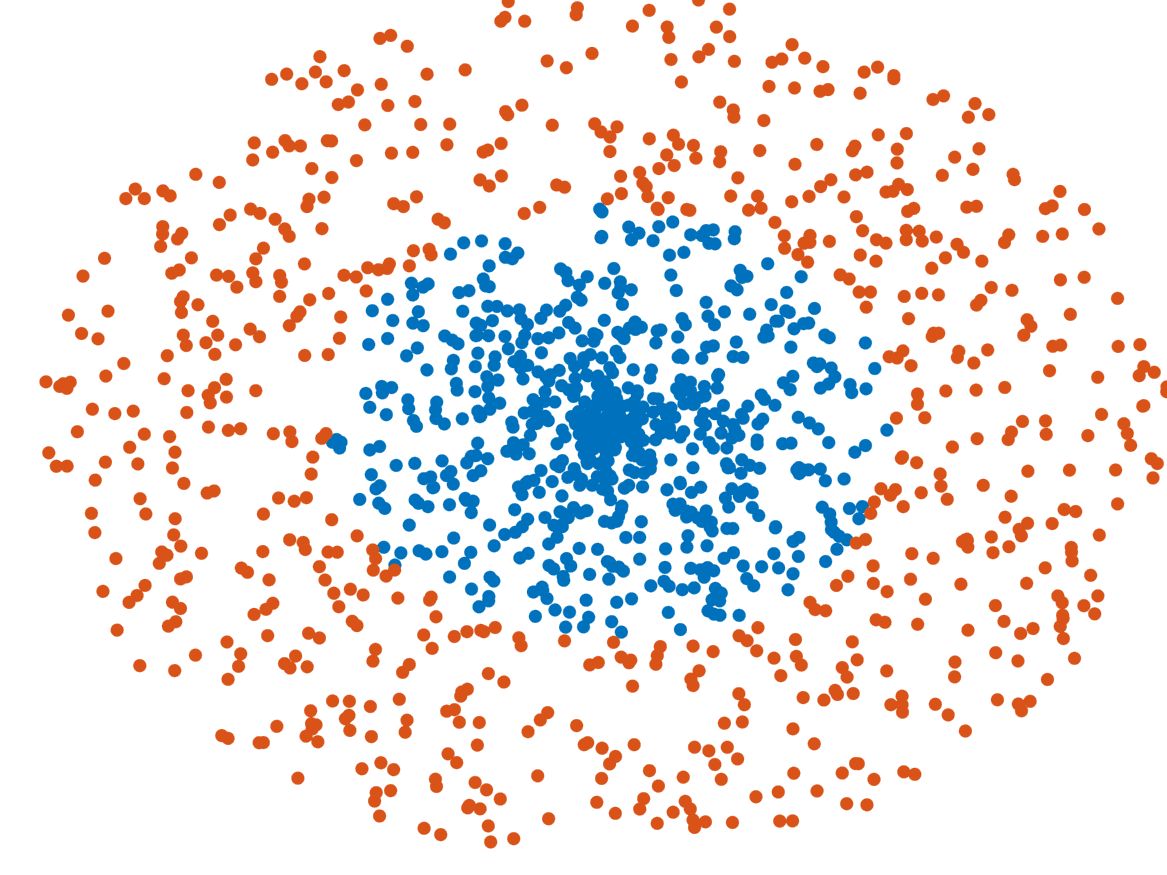
\includegraphics[width=45mm]{Circle-train} & 
		\invisible<beamer|1>{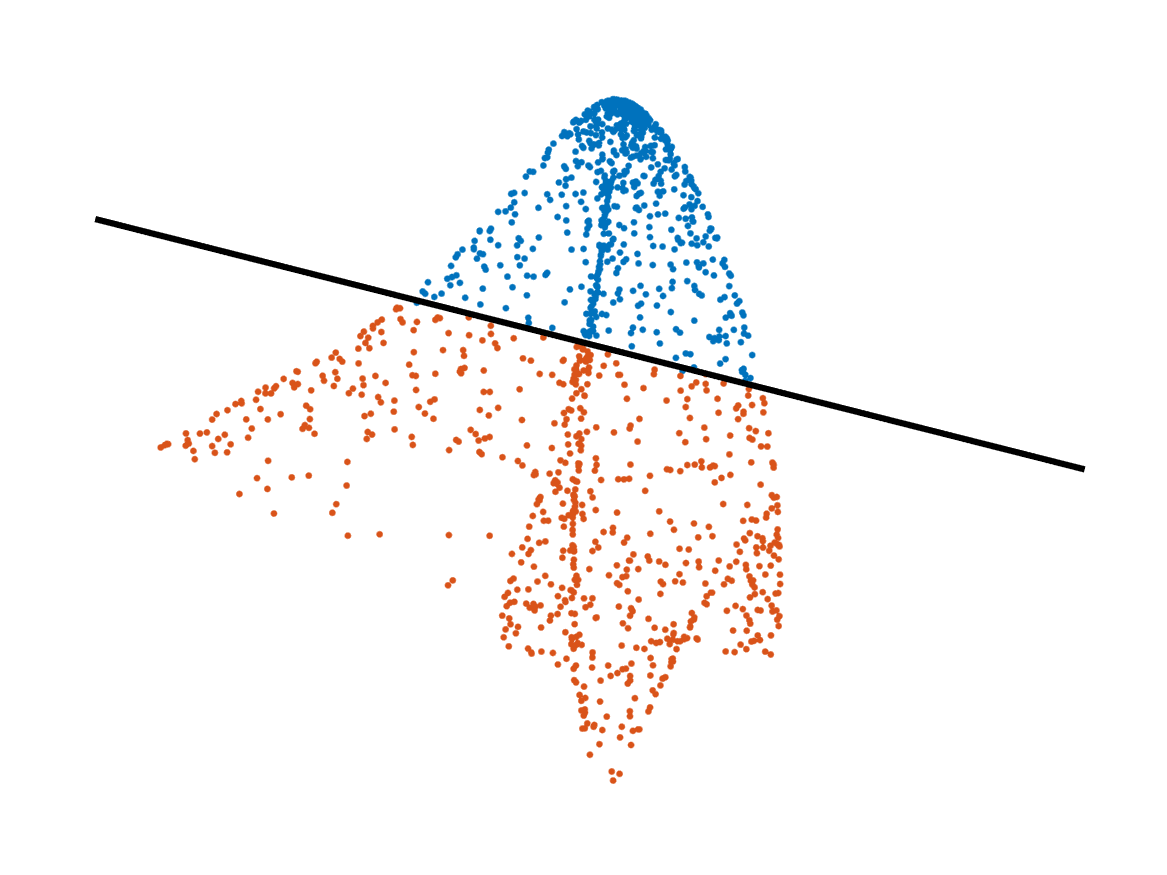
\includegraphics[width=45mm]{Circle-proptrain} }\\
		input features & \invisible<beamer|1>{transformed features}
	\end{tabular}
\end{center}

\bigskip

\invisible<beamer|1>{{\bf Goal/Trick}

Embed the points in higher dimension and/or move the points to make them
linearly separable}

\only<beamer|2>{}
\end{frame}

\begin{frame}\frametitle{Motivation: Nonlinear Models}


In general, impossible to find a linear separator between classes
%$$ \bfC = \bfX \bfW + b $$

\begin{center}
	\begin{tabular}{cc}
		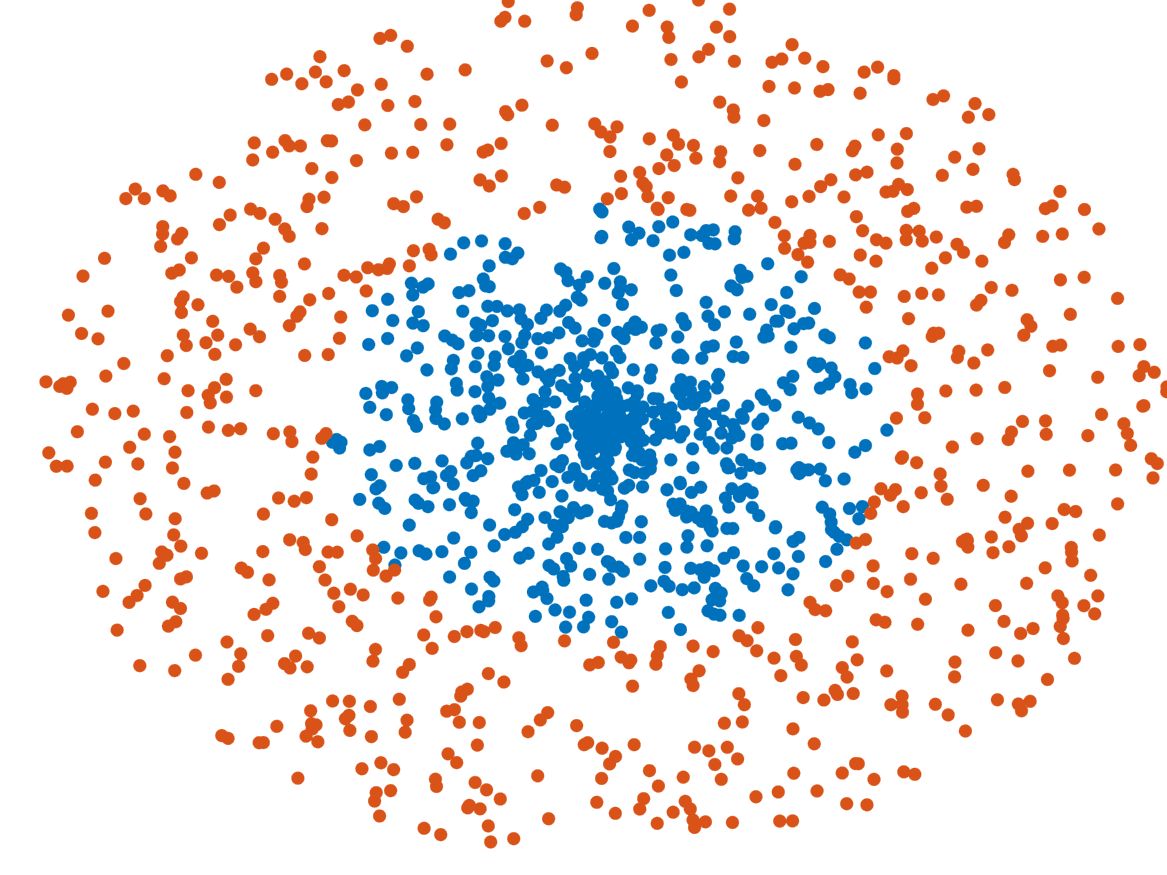
\includegraphics[width=45mm]{Circle-train} & 
		\invisible<beamer|1>{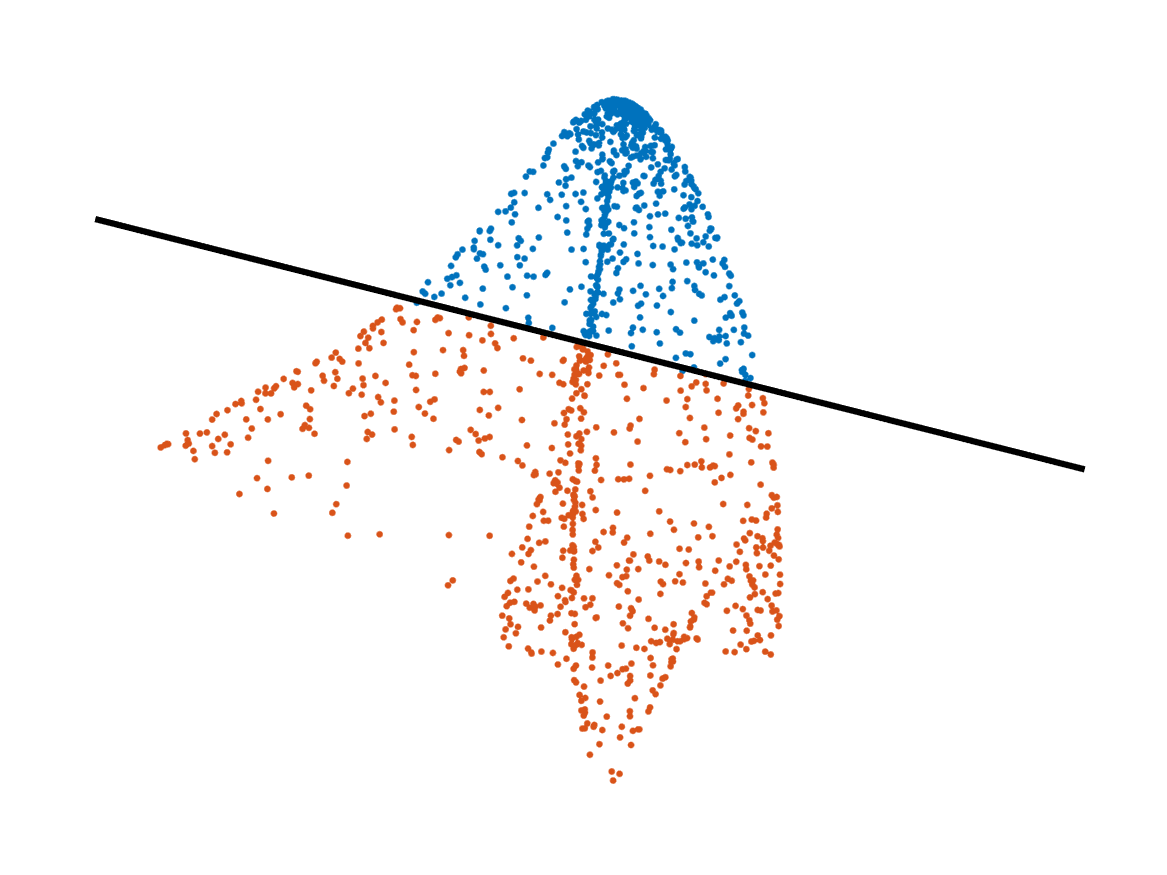
\includegraphics[width=45mm]{Circle-proptrain} }\\
		input features & \invisible<beamer|1>{transformed features}
	\end{tabular}
\end{center}

\bigskip

\invisible<beamer|1>{{\bf Goal/Trick}

Embed the points in higher dimension and/or move the points to make them
linearly separable}

\only<beamer|2>{}
\end{frame}

\begin{frame}\frametitle{Example: Linear Fitting}


Assume $\bfC\in \R^{n_c\times n}$, $\bfY \in \R^{n_f \times n}$ and $n \gg n_f$.
Goal: Find $\bfW \in \R^{n_c \times n_f}$ such that

$$ \bfC = \bfW \bfY $$

\bigskip
\pause

If ${\rm rank}(\bfY)<n$, there may be no solution.

\bigskip
\pause

Two options:
\begin{enumerate}
	\item Regression: Solve $\min_\bfW \| \bfW \bfY - \bfC \|_F^2$ $\leadsto$ always has solutions, but residual might be large
	\item Nonlinear Model: Replace $\bfY$ by $\sigma(\bfK\bfY)$ in regression, where $\sigma$ is element-wise function (aka activation) and $\bfK \in \R^{m \times n_f}$ where $m \gg n_f$
\end{enumerate}

\end{frame}


\begin{frame}\frametitle{Illustrating Nonlinear Models}

\begin{center}
	\begin{tabular}{cc}
		\rotatebox{90}{original} & 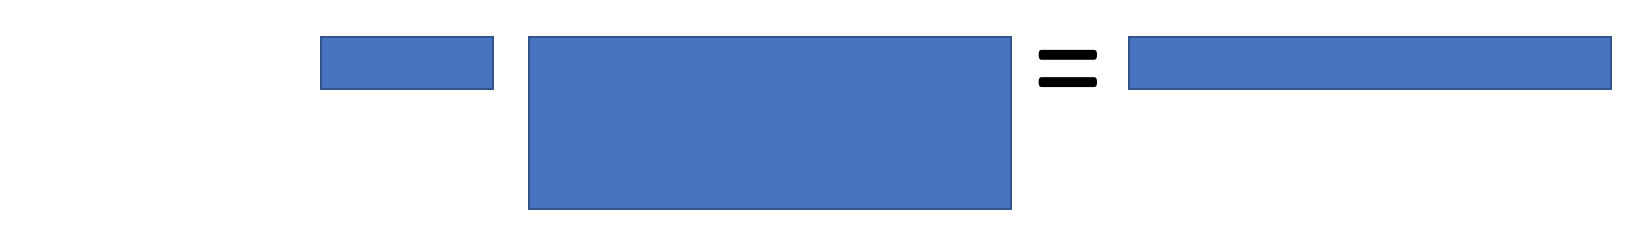
\includegraphics[width=.9\textwidth]{elmSmall}\\
		 \invisible<beamer|1>{\rotatebox{90}{transformed}} & 
		\invisible<beamer|1>{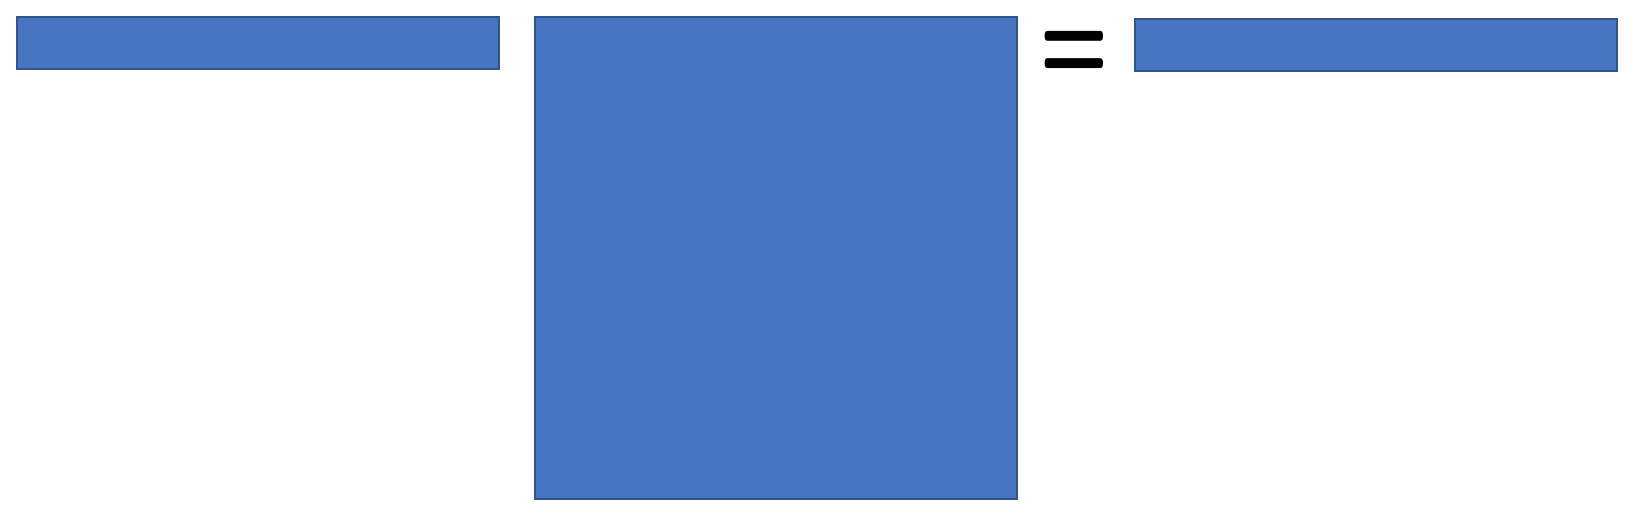
\includegraphics[width=.9\textwidth]{elmBig}}\\
	\end{tabular}
\end{center}

\bigskip

\invisible<beamer|1>{
Remarks
\begin{itemize}
	\item instead of $\bfW \bfY = \bfC$ solve $\hat{\bfW} \sigma(\bfK \bfY)  = \bfC$
	\item solve bigger problem $\leadsto$ memory, computation, \ldots
	\item what happens to ${\rm rank}(\sigma(\bfK\bfY))$ when $\sigma(x)=x$?
\end{itemize}}

\only<beamer|2>{}
\end{frame}




\begin{frame}[fragile]\frametitle{Conjecture: Universal Approximation Properties}

Given the data $\bfY \in \R^{n_f \times n}$ and $\bfC \in \R^{n_c \times n}$
with $n\gg n_f$, there is nonlinear function $\sigma:\R \to \R$, a matrix $\bfK \in \R^{m \times n_f}$, and a bias $\bfb \in \R^m$ such that

$$
 {\rm rank}(\sigma(\bfK \bfY + \bfb)) = n.
$$

\bigskip
\pause
Therefore, possible~\cite{Cybenko1989,HornikEtAl1989} to find ${\bfW}\in\R^{n_c\times m}$

$$\bfW \sigma( \bfK \bfY + \bfb) = \bfC.$$

\end{frame}


\begin{frame}[fragile]\frametitle{Choosing Nonlinear Model}

$$ \bfW  \sigma(\bfK \bfY+ \bfb)= \bfC $$
\begin{itemize}
\item how to choose $\sigma$?
\pause
\begin{itemize}
	\item early days: motivated by neurons
	\item popular choice: $\sigma(x) = \tanh(x)$ (smooth, bounded, \ldots)
	\item nowadays: $\sigma(x) = \max(x,0)$ (aka ReLU, rectified linear unit, non-differentiable, not bounded, simple)
\end{itemize}
\pause
\item how to choose $\bfK$ and $\bfb$?
\pause
\begin{itemize}
	\item pick randomly $\leadsto$ branded as \emph{extreme learning machines}~\cite{HuangEtAl2006}
	\item train (optimize) $\leadsto$ done for most neural network
	\item \emph{deep learning} when neural network has many layers
\end{itemize}
\end{itemize}


\end{frame}

\begin{frame}\frametitle{First Experiment: Random Transformation}

Select activation function and choose $\bfK$ and $\bfb$ randomly and solve the least-squares/classification problem

\bigskip

The Pros:
\begin{itemize}
\item universal approximation theorem: can interpolate any function
\item very(!) easy to program
\item can serve as a benchmark to more sophisticated methods
\end{itemize}

\bigskip

Some concerns:
\begin{itemize}
\item may require very large $\bfK$ (scale with $n$, number of examples)
\item may not generalize well
\item large dense linear algebra
\end{itemize}

\begin{center}
	\texttt{EELM\_Peaks.m}
\end{center}
\end{frame}

\begin{frame}[fragile]\frametitle{Learning the Weights}

Assume that the number of examples, $n$, is very large.

Using random weights, $\bfK$ might need to be very large to fit training data.

Solution may not generalize well to test data.

\bigskip
\pause

Idea: Learn $\bfK$ and $b$  from the data (in addition to $\bfW$)

$$ \min_{\bfK,\bfW,b} E(\bfW\sigma(\bfK \bfY + \bfb), \bfC^{\rm obs}) + \lambda R(\bfW,\bfK,\bfb)$$

About this optimization problem:
\begin{itemize}
	\item more unknowns $\bfK \in \R^{m \times n_f}$, $\bfW \in \R^{n_c \times m}$, $\bfb \in \R^m$
	\item  non-convex problem $\leadsto$ local minima, careful initialization
	\item need to compute derivatives w.r.t. $\bfK, \bfb$
\end{itemize}


\end{frame}


\begin{frame}
	\frametitle{Non-Convexity}
	The optimization problem is non-convex. Simple illustration of cross-entropy along two random directions $d\bfK$ and $d\bfW$

	\begin{center}
		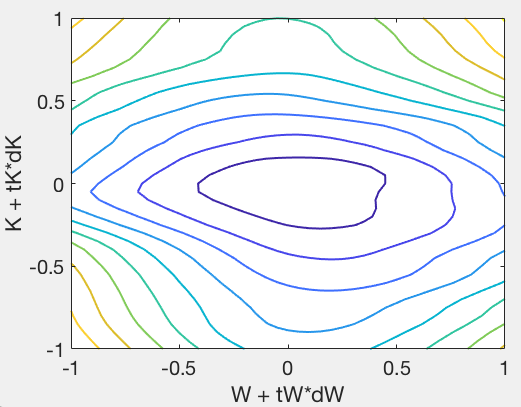
\includegraphics[width=.6\textwidth]{nonConvexitySingleLayer}
		
		(see \texttt{ESingleLayer\_PlotObjective.m})
	\bigskip
	
	Expect worse when number of layers grows!
	\end{center}

\end{frame}
\begin{frame}[fragile]\frametitle{Training the Neural Network}

\begin{itemize}
\item If non-convexity is not ``too bad'' can use standard gradient based methods
\item If non-convexity is ``ugly'' need to modify standard methods (stochastic kick)
\item If non-convexity is ``bad'' need global optimization techniques
\end{itemize}

	\begin{center}
	\begin{tabular}{ccc}
		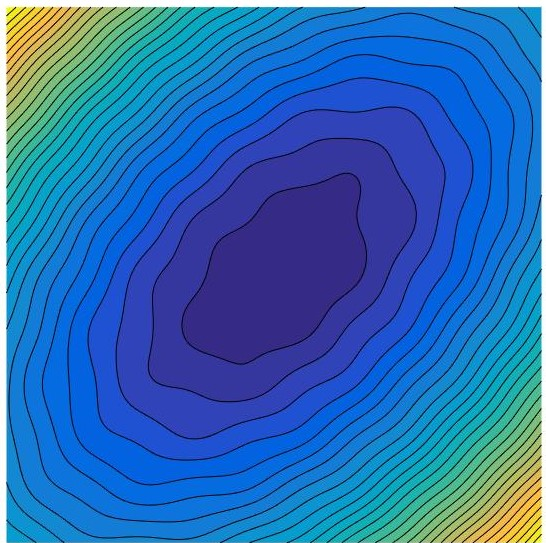
\includegraphics[width=.3\textwidth]{images/goodConv} &
		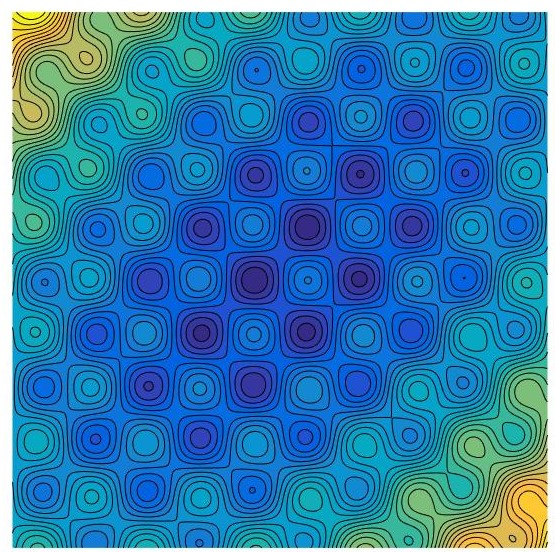
\includegraphics[width=.3\textwidth]{images/badConv} &
		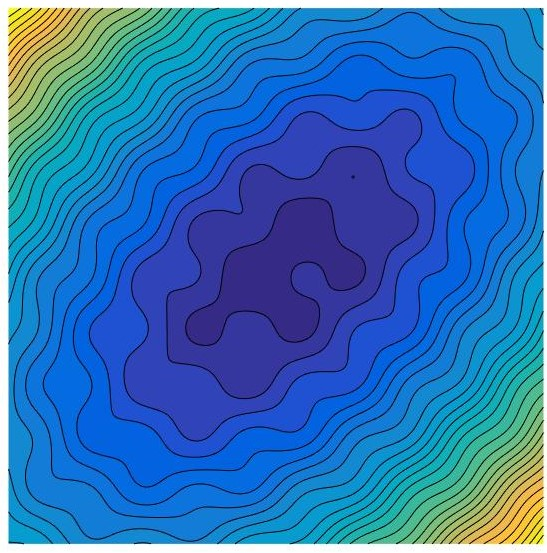
\includegraphics[width=.3\textwidth]{images/uglyConv} \\
		good & bad & ugly \\
		\end{tabular}
		\end{center}



\end{frame}
\begin{frame}[fragile]\frametitle{Recap: Differentiating Linear Algebra Expressions}

Easy ones:
\begin{align*}
 F_1(\bfx,\bfy) &= \bfx^{\top} \bfy  & \bfJ_{\bfx}F_1(\bfx,\bfy) = \bfy^\top\\
F_2(\bfA,\bfx)  &= \bfA \bfx         & \bfJ_{\bfx}F_2(\bfx,\bfy) = \bfA 
\end{align*}
\pause
How about
$$ F_3(\bfA,\bfX) =   \bfA  \bfX \quad \quad \bfJ_{{\rm vec}(\bfX)}F_3 = ??? $$
\pause
Recall that
$${\rm vec}(\bfA \bfX) = {\rm vec}(\bfA  \bfX \bfI) = (\bfI \otimes \bfA) {\rm vec} (\bfX) $$
Therefore:
$$ \bfJ_{{\rm vec}(\bfX)}F_3(\bfA,\bfX) = \bfI \otimes \bfA $$
\pause
\textcolor{red}{
Efficient mat-vec: } $\bfJ_{{\rm vec}(\bfX)}F \bfv = {\rm vec} ( { \bfA\ \rm mat}(\bfv) )$
	
\end{frame}


\begin{frame}[fragile]\frametitle{Training Single Layer Neural Network}

Assume no regularization (easy to add) and re-write optimization problem as 
\begin{eqnarray*}
 \min_{\bfW,\bfK,b}  E(\bfC^{\rm obs}, \bfZ,\bfW ) \quad \text{ with} \quad \bfZ = \sigma(\bfK\bfY + b)
\end{eqnarray*}

\bigskip
\pause

Agenda:
\begin{enumerate}
	\item compute derivative of ${\rm vec}(\bfZ)$ w.r.t. ${\rm vec}(\bfK), b$ 
	\item use chain rule to get
	\begin{align*}
		\bfJ_{{\rm vec}(\bfK)} E  & = \bfJ_{{\rm vec}(\bfZ)} E(\bfC^{\rm obs},\bfZ,\bfW) \ \bfJ_{{\rm vec}(\bfK)} \bfZ\\
		\bfJ_{b} E  & = \bfJ_{{\rm vec}(\bfZ)} E(\bfC^{\rm obs},\bfZ,\bfW) \ \bfJ_{b} \bfZ
	\end{align*}
	\item efficient code for mat-vecs with $\bfJ$ and $\bfJ^\top$
\end{enumerate} 
\end{frame}

\begin{frame}[fragile]\frametitle{Computing Jacobians}
$$
\bfZ = \sigma(\bfK\bfY + b)
$$
Recall that $\sigma$ is applied element-wise.
$$
	\bfJ_{{\rm vec}(\bfK)}\bfZ = {\rm diag}(\sigma'(\bfK \bfY + b)) (\bfY^\top \otimes \bfI)
$$
\pause
Efficient way to get matrix vector products
\begin{eqnarray*}
\bfJ_{{\rm vec}(\bfK)}\bfZ \bfv &=& {\rm diag}(\sigma'(\bfK \bfY + b)) (\bfY^\top \otimes \bfI)\bfv\\
                            &=& {\rm vec} \left(\sigma'(\bfK \bfY + b) \odot ( {\rm mat}(\bfv) \bfY )\right)
\end{eqnarray*}
And for transpose get
\begin{eqnarray*}
(\bfJ_{{\rm vec}(\bfK)}\bfZ)^\top \bfu &=& (\bfY \otimes \bfI) {\rm diag}(\sigma'(\bfK \bfY + b)) \bfu\\
                            &=& {\rm vec} \left(\sigma'(\bfK \bfY + b) \odot  {\rm mat}(\bfu)\bfY^\top\right) 
\end{eqnarray*}

\end{frame}




\begin{frame}[fragile]\frametitle{Class Problems: Derivatives of Single Layer}

\textbf{Derivations:}
\begin{enumerate}
	
	\item Compute $\bfJ_{b}\bfZ v$ and $(\bfJ_{b}\bfZ)^\top \bfu$

	\item Compute $\bfJ_{{\rm vec}(\bfY)}\bfZ  \bfv$ and $(\bfJ_{{\rm vec}(\bfY)}\bfZ)^\top  \bfu$
\end{enumerate}

\textbf{Coding:}
\begin{verbatim}
function[Z,JKt,Jbt,JYt,JK,Jb,JY] = singleLayer(K,b,Y)
% Returns Z = sigma(K*Y+b) and 
%                         functions for J'*U and J*V
\end{verbatim}

\textbf{Testing:}
\begin{enumerate}
	\item Derivative check for Jacobian mat-vec
	\item Adjoint tests for transpose, let $\bfv,\bfu$ be arbitray vectors
	$$
		\bfu^\top \bfJ \bfv \approx \bfv^\top \bfJ^\top \bfu
	$$
\end{enumerate}

\end{frame}


\begin{frame}[fragile]
	\frametitle{Putting Things Together}
	
	Implement loss function of single-layer NN
	$$
		E(\bfK,b,\bfW) \stackrel{def}{=} E(\bfC,\bfZ,\bfW), \quad \bfZ = \sigma(\bfK \bfY+b)
	$$
	
	
	\begin{verbatim}
		function [Ec,dE] = singleLayerNNObjFun(x,Y,C,m)
		% where x = [K(:); b; W(:)]
		% evaluates single layer and computes cross entropy 
		%        and gradient (extend for approx. Hessian)
	\end{verbatim}

	\bigskip
	
    Use
	\begin{enumerate}
		\item $\nabla_{\bfZ} E =  \bfW^\top \nabla_{\bfS} \ E(\bfS), \quad \bfS = \bfW\bfZ$
		\item $\nabla_{\bfK} E =  \bfJ_{\bfK}^\top \nabla_{\bfZ} E$
		\item $\nabla_{\bfb} E =  \bfJ_{\bfb}^\top \nabla_{\bfZ} E$
		\item $\nabla_{\bfW} E =  \nabla_{\bfS} \ E(\bfS) \bfY $
	\end{enumerate}
	
	
\end{frame}

\begin{frame}[fragile]
	\frametitle{Test Problem}
	
	Before going to real data, let us try the \emph{inverse crime}. Generate data
	\begin{verbatim}
		n  = 500; nf = 50; nc = 10; m  = 40;
		Wtrue = randn(nc,m);
		Ktrue = randn(m,nf);
		btrue = .1;

		Y     = randn(nf,n);
		Cobs  = exp(Wtrue*singleLayer(Ktrue,btrue,Y));
		Cobs  = Cobs./sum(Cobs,1);		
	\end{verbatim}
	
	\begin{center}
	Goal: Reconstruct \texttt{Wtrue, Ktrue, btrue}!  
	\end{center}
\end{frame}

\begin{frame}
	\frametitle{Gauss-Newton Method}
	
	\textbf{Goal:} Use curvature information for fast convergence
	$$
	\nabla_{\bfK} E(\bfK,\bfb,\bfW) =  (\bfJ_\bfK \bfZ)^\top \nabla_\bfZ E(\bfW\sigma(\bfK \bfY+\bfb),\bfC),
	$$
	where $\bfJ_\bfK \bfZ = \nabla_{\bfK} \sigma(\bfK \bfY+\bfb)^\top$.\pause This means that Hessian is
	\begin{equation*}
		\begin{split}
	\nabla_{\bfK}^2 E(\bfK) &  = (\bfJ_{\bfK}\bfZ)^\top  \nabla_\bfZ^2 E(\bfC,\bfZ,\bfW) \bfJ_{\bfK}\bfZ\\
	 & + \sum_{i=1}^{n}\sum_{j=1}^{m} \nabla_{\bfK}^2 \sigma(\bfK \bfY+\bfb)_{ij} \nabla_\bfZ E(\bfC,\bfZ,\bfW)_{ij}
		\end{split}
	\end{equation*}
	
	First term is spsd and we can compute it.
	
	\pause
	
	We neglect second term since
	\begin{itemize}
		\item can be indefinite and difficult to compute
		\item small if transformation is roughly linear or close to solution (easy to see for least-squares)
	\end{itemize}
	\begin{center}
		\textcolor{red}{do the same for $\bfb$ and use full Hessian for $\bfW$ $\leadsto$ ignore coupling!}
	\end{center}	
\end{frame}

\begin{frame}[fragile]
	\frametitle{Experiment: Adversarial Example}
	
	Suppose you have trained your network $\leadsto \bfK, b, \bfW$ so that validation loss is low. This means that for most examples $\bfy$, 
	$$
		\bfW \sigma(\bfK \bfy + b) \approx \bfc.
	$$
	
	An adversary might try to fool this classifier by adding a small perturbation $\bfd$ to the example to achieve a desired label $\hat{\bfc}$. 
	
	\bigskip
	
	Formulate as optimization problem
	$$
		\min_{\bfd} E(\bfW \sigma(\bfK (\bfy + \bfd) + b), \hat{\bfc})
	$$
	\begin{itemize}
		\item setup objective function
		\item think about constraints, regularization
	\end{itemize}
\end{frame}


\end{document}
\begin{frame}[fragile]\frametitle{Learning the weights}

{\bf Class problem}

\bigskip


Code a function
\small
\end{frame}


\begin{frame}[fragile]\frametitle{Overview}

Given data $\bfY \in \R^{n_f\times n}$ and class probabilities $\bfC\in\R^{n_c\times n}$ we aim to find the transformation parameters $\bftheta\in\R^p$ and classification weights (including potentially biases) $\bfW \in \R^{n_c \times m}$ by solving
$$
\min_{\bftheta,\bfW} E(\bfW \sigma(\bfK(\bftheta)\bfY), \bfC) + \lambda R(\bftheta,\bfW)
$$

Today: Derive practical pipeline consisting of 
\begin{itemize}
	\item variable projection
	\item Stochastic Average Approximation (SAA)
	\item regularization
\end{itemize}


\end{frame}

\begin{frame}\frametitle{Variable Projection - 1}
	Idea: Treat learning problem as coupled optimization problem with blocks $\bftheta=(\bfK,\bfb)$ and $\bfW$. 
	
	Simple illustration for coupled least-squares problem~\cite{GoPe1973,GoPe03,OLearyRust2013}
	$$
		\min_{\bftheta,\bfw} \phi(\bftheta,\bfw) = \hf \| \bfA(\bftheta) \bfw - \bfc\|^2 + \frac{\lambda}{2}\| \bfL \bfw\|^2 + \frac{\beta}{2} \| \bfM \bftheta\|^2
	$$
	
	\pause
	
	Note that for given $\bftheta$ the problem becomes a standard least-squares problem. Define: 
	$$
		\bfw(\bftheta) = \left( \bfA(\bftheta)^\top \bfA(\bftheta) + \lambda \bfL^\top \bfL \right)^{-1}{\bfA(\bftheta)^\top \bfc}
	$$
	
	\pause
	This gives optimization problem in $\bftheta$ only (aka \emph{reduced/projected  problem})
	$$
		\min_{\bftheta} \tilde{\phi}(\bftheta) = \hf \| \bfA(\bftheta) \bfw(\bftheta) - \bfc\|^2 + \frac{\lambda}{2}\| \bfL \bfw(\bftheta)\|^2 + \frac{\beta}{2} \| \bfM \bftheta\|^2
	$$
	
\end{frame}
\begin{frame}\frametitle{Variable Projection - 2}
	$$
		\min_{\bftheta} \tilde{\phi}(\bftheta) = \hf \| \bfA(\bftheta) \bfw(\bftheta) - \bfc\|^2 + \frac{\lambda}{2}\| \bfL \bfw(\bftheta)\|^2 + \frac{\beta}{2} \| \bfM \bftheta\|^2
	$$
	Optimality condition:
	$$ 
		\nabla \tilde{\phi}(\bftheta) = \nabla_\bftheta \phi(\bftheta,\bfw) + \nabla_\bftheta \bfw(\bftheta) \nabla_{\bfw} \phi(\bftheta,\bfw) \stackrel{!}{=} 0.
	$$
	Less complicated than it seems since
	$$
		\nabla_{\bfw} \phi(\bftheta,\bfw(\bftheta)) = \bfA(\bftheta)^\top( \bfA(\bftheta) \bfw(\bftheta) - \bfc) + \lambda \bfL^\top \bfL \bfw(\bftheta) = 0
	$$
	
	Discussion:
	\begin{itemize}
		\item ignore second term in gradient computation
		\item apply gradient descent/NLCG/BFGS  to minimize $\tilde{\phi}$
		\item solve least-squares problem in each evaluation of $\tilde{\phi}$
		\item gradient is only correct if LS problem is solved exactly
	\end{itemize}
	
\end{frame}

\begin{frame}
	\frametitle{Variable Projection for Single Layer}
	
$$
\min_{\bftheta,\bfW} E(\bfW \sigma(\bfK(\bftheta)\bfY ), \bfC) + \lambda R(\bftheta,\bfW)
$$
Assume that the regularizer is separable, i.e.,
$$
 R(\bftheta,\bfW) =   R_1(\bftheta) +  R_2(\bfW)
$$
and that $R_2$ is convex and smooth. 
\pause
Hence, the projection requires solving the regularized classification problem
$$
\bfW(\bftheta) = \argmin_{\bfW} E(\bfW\sigma(\bfK(\bftheta)\bfY), \bfC) + \lambda R_2(\bfW)
$$
practical considerations:
\begin{itemize}
	\item solve for $\bfW(\bftheta)$ using Newton (need accuracy)
	\item need good solver to approximate gradient w.r.t. $\bftheta$  well
	\item use Gauss-Newton or steepest descent to solve for $\bftheta$ 
\end{itemize}
\end{frame}

\begin{frame}\frametitle{Stochastic Optimization}
	Assume that each $\bfy_i$, $\bfc_i$ pair is drawn from some (unknown probability distribution). 
	
	Then, we can interpret the learning problem as minimizing the expected value of the cross entropy, e.g., in linear regression
	$$
		E(\bftheta,\bfW) = {\mathbb{E}} \left(\hf \|\bfW \sigma(\bfK(\bftheta)\bfy + \bfb ) - \bfc\|^2\right)
	$$
	
	This is a stochastic optimization problem~\cite{bottou2016optimization}. \pause One idea: \textbf{Stochastic Approximation: } Design iteration $(\bftheta_k,\bfW_k) \to (\bftheta^*,\bfW^*)$ so that expected value decreases.
		
		Example: Stochastic Gradient Descent, ADAM, \ldots
		
		Pro: sample can be small (\emph{mini batch})
		
		Con: how to monitor objective, linesearch, descent, \ldots
\end{frame}
\begin{frame}[fragile]\frametitle{Review: Supervised Learning Problem}

Most machine learning problems are of the following structure
$$
\min_{\bftheta} F(\bftheta,\bfY) + R(\bftheta), \quad \text{ with }\quad  F(\bftheta,\bfY) = \frac1n\sum_{i=1}^n f_i(\bftheta,\bfy_i).
$$

\bigskip
\pause

For shallow learning, problem might be convex or have a unique minimum.
For deep networks, problem is usually not convex and has many local minimum

\end{frame}

\begin{frame}[fragile]\frametitle{Review - Optimization Techniques}

So far, we used deterministic gradient-based methods
$$ \bftheta_{k+1} = \bftheta_k - \mu_k \bfA_k^{-1} \grad F(\bftheta_k,\bfY), \quad  \nabla F(\bftheta,\bfY) = \frac1n  \sum_{i=1}^n \nabla f_i(\bftheta, \bfy_i)$$

\smallskip 
\pause

Examples: 
\begin{itemize}
	\item steepest descent: $ \bfA_k = \bfI$
	\item Newton: $\bfA_k = \nabla^{2} F(\bftheta,\bfY) = \sum_{i=1}^N \nabla^{2} f_i(\bftheta, \bfy_i)$
\end{itemize}

\bigskip
\pause

Drawbacks:
\begin{itemize}
\item
Evaluating gradient needs pass through the whole data set (called \emph{epoch}).
\item
If data is redundant can be very expensive
\item 
Idea: use only a part of the data to update $\bftheta$
\end{itemize} 



\end{frame}


\begin{frame}[fragile]\frametitle{Stochastic Gradient Descent}

Let ${\cal S}_k \subset \{1,2,\ldots,n\}$. Define the batch objective function as 
$$ F_{{\cal S}_k}(\bftheta) = \frac{1}{|{\cal S}_k|} \sum_{i \in {\cal S}_k} f_i(\bftheta,\bfY_i) $$
Then a straight forward extension  is
$$ \bftheta_{k+1} = \bftheta_k - \mu_k \bfA_k^{-1}  \grad F_{{\cal S}_k}(\bftheta_k) $$


Questions
\begin{itemize}
\item Would the method converge?
\item Under what conditions on $\mu_k,\bfA_k,{\cal S}_k$?
\item How fast?
\end{itemize}

References: original method~\cite{RobbinsMonro1951}, recent surveys~\cite{Bottou2012,Bertsekas2015,bottou2016optimization}
\end{frame}

\begin{frame}[fragile]\frametitle{Stochastic Gradient Descent}

Let ${\cal S}_k \subset \{1,2,\ldots,n\}$. Define the batch objective function as 
$$ F_{{\cal S}_k}(\bftheta) = \frac{1}{|{\cal S}_k|} \sum_{i \in {\cal S}_k} f_i(\bftheta,\bfY_i) $$
Then a straight forward extension   is
$$ \bftheta_{k+1} = \bftheta_k - \mu_k \bfA_k^{-1}  \grad F_{{\cal S}_k}(\bftheta_k) $$

\bigskip
\pause

If $\bfA_k = \bfI$, $|{\cal S}_k|=1$ and $\mu_k \rightarrow 0$ slow enough, that is
$$ \sum_{k=1}^{\infty} \mu_k= \infty \quad \text{ and } \quad \sum_{k=1}^{\infty} \mu_k^2 < \infty$$
then SGD converges to stationary point \pause (Ex: $\mu_k = k^{-1}$).

\bigskip
\pause

How fast? Convergence is {\bf sublinear}

\end{frame}


\begin{frame}\frametitle{A Glimpse into the theory}
	Consider the iteration and $\bfA_k=\bfI$
	$$ 
	\bftheta_{k+1} = \bftheta_k - \mu_k  \grad F_{{\cal S}_k}(\bftheta_k) 
	$$
	\pause
	Re-write this as
	$$ 
	\bftheta_{k+1} = \bftheta_k - \underbrace{\mu_k \grad F(\bftheta,\bfY)}_{\rm true\ gradient} -  \underbrace{\mu_k \left ( \grad F_{{\cal S}_k}(\bftheta_k)  - \grad F (\bftheta,\bfY)\right)}_{\rm noise}
	$$
	
	\pause
	
	Note that (unbiased estimator)
	$$
	 {\mathbb{E}} (\grad F_{{\cal S}_k}(\bftheta_k)) = \grad F (\bftheta).
	$$
	
	\pause
	
	Finally note that
	$$
		{\rm Var}\left( \mu_k \grad F_{{\cal S}_k}(\bftheta_k) \right) = \mu_k^2 {\rm Var}\left( \grad F_{{\cal S}_k}(\bftheta_k) \right)
	$$
\end{frame}

\begin{frame}[fragile]\frametitle{Improvements of SGD: Momentum}

Idea: Accelerate convergence by keeping gradient informations from previous batches.


\begin{eqnarray*}
&& \bfS_{k+1} = \gamma \bfS_k  +\mu_k  \grad F_{{\cal S}_k}(\bftheta_k) \\
&& \bftheta_{k+1} = \bftheta_k  - \bfS_{k+1}
\end{eqnarray*}
$\mu_k$ - learning rate, $\gamma$ - momentum 


\bigskip
\pause

Hard to choose in practice, heuristic

$\gamma$ - Start with $0.5$ and increase slowly to 0.9

$\mu$ - problem dependent start small and decrease after a few epoch


\end{frame}

\begin{frame}\frametitle{Improvements of SGD: Nesterov}

	Idea: Predict next iterate using momentum, correct next step using gradient there.
	
	\begin{eqnarray*}
	&& \bftheta_{k+\frac 12} = \bftheta_k  - \gamma \bfS_{k} \\
	&& \bfS_{k+1} = \gamma \bfS_k  + \mu_k  \grad F_{{\cal S}_k}({\bftheta_{k+\frac12}}) \\
	&& \bftheta_{k+1} = \bftheta_k  - \bfS_{k+1}
	\end{eqnarray*}
\end{frame}

\begin{frame}
	\frametitle{Improvements of SGD: AdaGrad}
	
	Idea: Scale step according to size of weights (relation to prior-conditioning in SGD)
	
	\bigskip
	
	
	Iteration:
	\begin{eqnarray*}
	&& \bfD_{k+1} = \bftheta_k^2 + \bfD_k \\
	&& \bfS_{k+1} =  \mu_k {\rm diag}(\bfD_{k+1})^{-1} \grad F_{{\cal S}_k}(\bftheta_{k}) \\
	&& \bftheta_{k+1} = \bftheta_k  - \bfS_{k+1}
	\end{eqnarray*}
	
	
\end{frame}

\begin{frame}[fragile]\frametitle{Theory and Final Comments}

General Comments:
\begin{itemize}
\item 
Lots of theory for convex problems
\item
Recall: SGD is not the best tool for most convex problems (see example of least-squares)
\item
Require very careful tuning
\end{itemize}

\bigskip

SGD in deep learning:
\begin{itemize}
	\item currently the main workhorse (DNN $\leadsto$ nonconvex optimization)
	\item why it works? mostly open but some relation to Langevin flow (we also have a few ideas)
	\item observed to regularize problems (theory for quadratic case)
	\item potentially possible to prove global optimality?
\end{itemize}
\end{frame}

\begin{frame}
	\frametitle{Coding: Using SGD for Classification Problem}
	
	Outline:
	\begin{itemize}
		\item Use single layer or ResNet example
		\item Change objective function to accept index set $S_k$
		\item Use small minibatch
		\item Test using peaks example
	\end{itemize}
\end{frame}

\begin{frame}
	\frametitle{Stochastic Average Approximation}
	
	Alternative way to solve stochastic optimization problem
	$$
	E(\bfW) = {\mathbb{E}} \left(\hf \| \bfW \sigma(\bfK(\bftheta)\bfy + \bfb) - \bfc\|^2\right)
	$$
	
	 Pick relatively large sample $S \subset \{ 1,\ldots,n\}$ and use deterministic optimization method to solve
			$$
				\min_{\bftheta,\bfW}  \frac{1}{2|S|} \sum_{s\in S} \| \bfW \sigma(\bfK(\bftheta)\bfy_s + \bfb )  - \bfc_s^\top \|^2.
			$$
		
			Pro: use your favorite solver, linesearch, stopping\ldots
			
			Con: large batches needed
			
			\begin{center}
				Note: Sample stays fixed during iteration.
			\end{center}
\end{frame}

\begin{frame}
	\frametitle{A Practical Approach}
	
	Let's combine VarPro and SAA to come up with a simple yet powerful training algorithm.
	
	\bigskip
	\pause
	
	Pick $(\bftheta_0)$ randomly and then do one or more steps of:
	\begin{enumerate}
		\item randomly select samples $S$ (large enough)
		\item do a few steps of variable projection to get $\bftheta_k$.
		\begin{itemize}
			\item inner solver: a few steps of Newton's method
		\end{itemize}
		\item check training error on current batch and validation error
	\end{enumerate}
	
	\bigskip
	\pause
	
	Possible problems:
	\begin{itemize}
		\item $|S|$ too small $\rightarrow$ training error small but no convergence
		\item $|S|$ too large $\rightarrow$ slow, overfitting (use regularization)
		\item Too few Newton steps in classification $\rightarrow$ inaccurate gradients, line search fails, \ldots
	\end{itemize}	
\end{frame}

\begin{frame}[fragile]\frametitle{Data Preprocessing}

Some practical tips
\begin{itemize}
\item Remove the mean of the data
\item Scale it to be ``reasonable'' scale
\item Data augmentation
\item Some other (domain specific) data transforms (optical flow for motion?)
\end{itemize}

\end{frame}

\begin{frame}[fragile]\frametitle{Regularization for Network Weights}

\begin{itemize}
\item
Note that there are many more degrees of freedom.
\item
Need to add regularization for $\bfK$
\item
$\bfK$ Generally, $\bfK$ is not ``physical'' - difficult to choose reasonable
regularization.
\end{itemize}

\bigskip

The obvious choice: Tikhonov
$$ R(\bfK) = \hf \|\bfK\|^2_F $$
(also called weight decay)


\end{frame}

\begin{frame}[fragile]\frametitle{Learning the weights - Regularization}

\begin{columns}
	\column{.7\textwidth}
More recent, demand that $\bfK$ is sparse
$$ R(\bfK) = \|{\rm vec}(\bfK)\|_1 = \sum_{ij} |\bfK_{ij}| $$

\bigskip

Implementation through soft-thresholding.


After each steepest descent iteration set
$$ \bfK = {\rm softThresh}(\bfK) $$
	
	\column{.3\textwidth}
	\begin{center}
	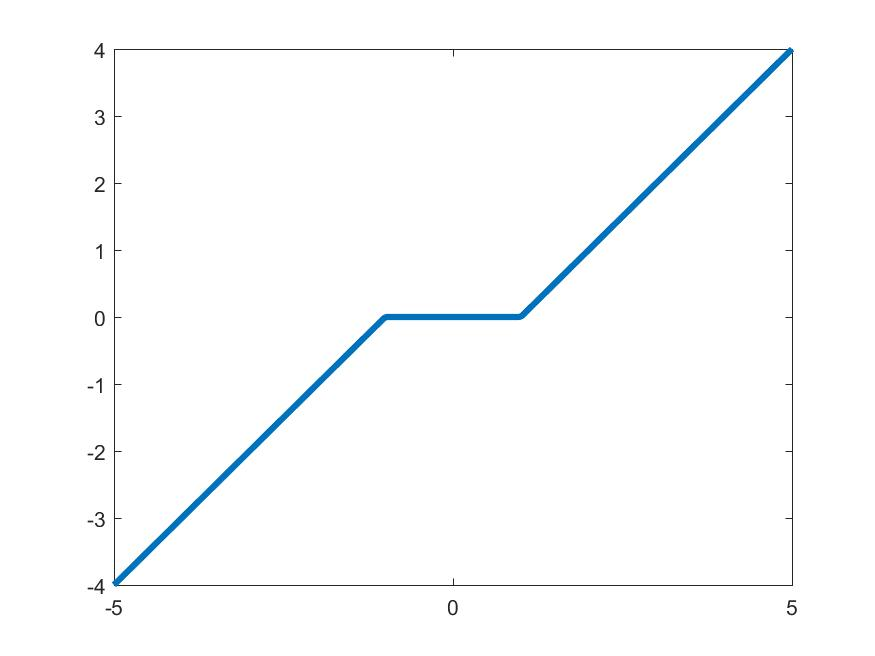
\includegraphics[width=4cm]{shoftThresh.jpg}
	\end{center}
	
\end{columns}

\vspace{10mm}
\begin{center}
Obtain sparse matrices $\bfK$ that retain only necessary entries
	
\end{center}

\end{frame}




\begin{frame}[fragile]\frametitle{Coding: Learning the weights }

{\bf Class problem}

\bigskip

Modify your steepest descent, nonlinear CG and SGD codes to work on single layer
network with soft thresholding.

Test on Circle, peaks, spiral, MNIST and CIFAR10

Compare and report

\end{frame}
\begin{frame}\frametitle{Experiment: Peaks}
	
	Compare the three approaches for training a single layer neural network
	
	\begin{itemize}
		\item \texttt{ESingleLayer\_PeaksSGD.m} - stochastic gradient descent 
		\item \texttt{ESingleLayer\_PeaksNewtonCG.m} - Newton CG with block-diagonal Hessian approximation
		\item \texttt{ESingleLayer\_PeaksVarPro.m} - Fully coupled solver. Eliminate $\bftheta$ and use steepest descent/Newton CG for reduced problem.
	\end{itemize}
	
\end{frame}

\begin{frame}[allowframebreaks]
	\frametitle{References}
\bibliographystyle{abbrv}
\bibliography{NumDNN}

\end{frame}



